\section{Results}
In this section, we shall see the results obtained after performing the Grover Search. Since we are using the \textbf{little-endian} system, the output qubits obtained must be read from right to left to get the ASCII value of the nonce-character. We will then append the nonce to the message and check if its classical hash indeed starts with $5$ zeroes when written in binary.

\subsubsection*{Number of Gates}
\noindent First we observe the difference in the number of gates used in the Grover and the Generalized Grover Search algorithms. To count the gates, we split them as follows\\

\noindent Each LFSR (or LFSR inverse) has\\
7 $SWAP$ gates\\
3 $CX$ gates\\

\noindent Each Diffuser has\\
18 $H$ gates\\
16 $X$ gates\\
1 $MCT$ gate\\

\noindent Each Generalized Diffuser has\\
16 $R_y$ gates\\
2 $H$ gates\\
1 $MCT$ gate\\

\noindent Each iteration has\\
2 LFSRs\\
2 Inverse LFSRs\\
1 Diffuser (or Generalized Diffuser)\\
16 $CX$ gates\\
10 $X$ gates\\
1 $MCT$ gate\\

There are 8 $H$ gates at the start followed by 4 iterations. Thus the total number of gates can be summarized by table \ref{Tab:7.1}.

\begin{table}[!htb]
\centering
	\begin{tabular}{|M{5cm}|M{1.5cm}|M{1.5cm}|M{1.5cm}|M{1.5cm}|M{1.5cm}|M{1.5cm}|M{2cm}|}
		\hline
		\multicolumn{8}{|c|}{\addmathvspace\textbf{SUMMARY OF THE NUMBER OF GATES USED}}\\
		\hline
		\addmathvspace\textbf{Algorithm} & 
		$\mathbf{H}$ &
		$\mathbf{X}$ &
		$\mathbf{CX}$ &
		$\mathbf{SWAP}$ &
		$\mathbf{MCT}$ & 
		$\mathbf{R_y}$ & 
		$\mathbf{TOTAL}$\\[5pt]
		\hline
		Grover Search&80&104&112&112&8&0&416\\[3pt]
		\hline
		Generalized Grover Search&16&40&112&112&8&64&352\\[3pt]
		\hline		
	\end{tabular}
	\caption{Table summarizing the number of gates required}
	\label{Tab:7.1}
\end{table}
\FloatBarrier
We observe that the Generalized Grover Search algorithm uses significantly less number of gates.

\subsubsection*{Qiskit Simulation}
\noindent Here, we will use the \textbf{aer\_simulator} provided by qiskit to run our code.
For testing purposes our message is\\
Message: \verb|Hello World|\\
This is then passed on to our program. A simulation of 1024 measurements is done. The result is shown in figure \ref{Fig:7.1}.
\begin{figure}[!htb]
   \begin{minipage}{\textwidth}
     \centering
     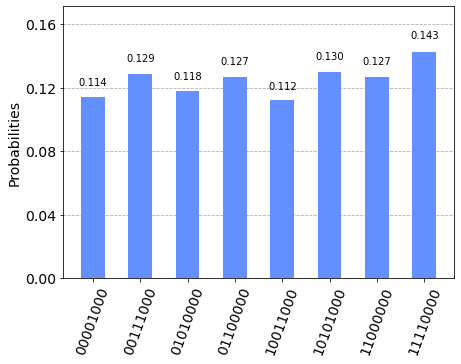
\includegraphics[scale=0.8]{fig07.01.png}
     \caption{Nonce values obtained and their probabilities}
     \label{Fig:7.1}
   \end{minipage}
\end{figure}
Note that since all since we are using the \textbf{little-endian} system, output must be read from right to left. Converting the binary to decimal, we get the ASCII of the nonce to be appended as \\

\begin{minipage}{\textwidth}
\begin{lstlisting}
28
3
21
25
15
6
10
16
\end{lstlisting}
\end{minipage}

We append the nonce and test the output hashes. The output hashes are (in the same order as the nonce values)\\

\begin{minipage}{\textwidth}
\begin{lstlisting}
4
3
6
5
0
2
1
7
\end{lstlisting}
\end{minipage}

Thus, we conclude that our algorithm works successfully.
